% =============================================================
% IEEE Conference Paper – Final Version
% Title: Subjective Novelty Detection for Automated EDA
% Author: Krishna Vamsi
% Format: IEEEtran (two-column conference)
% =============================================================

\documentclass[conference]{IEEEtran}
\IEEEoverridecommandlockouts

% ── Core packages ────────────────────────────────────────────
\usepackage{cite}
\usepackage{amsmath,amssymb,amsfonts}
\usepackage{algorithmic}
\usepackage{algorithm}
\usepackage{graphicx}
\usepackage{textcomp}
\usepackage{xcolor}
\DeclareGraphicsExtensions{.pdf,.png,.jpg,.jpeg}
\usepackage[hidelinks]{hyperref}
\usepackage{booktabs}
\usepackage{multirow}
\usepackage{array}
\usepackage{listings}
\usepackage{tikz}
\usepackage{pgfplots}
\pgfplotsset{compat=1.18}
\usetikzlibrary{shapes,arrows,positioning,fit,backgrounds}

% ── Code listing style ────────────────────────────────────────
\lstset{
  basicstyle=\ttfamily\scriptsize,
  breaklines=true,
  frame=single,
  keywordstyle=\color{blue}\bfseries,
  commentstyle=\color{gray},
  stringstyle=\color{orange!70!black},
  numbers=left,
  numberstyle=\tiny\color{gray},
  numbersep=4pt
}

\def\BibTeX{{\rm B\kern-.05em{\sc i\kern-.025em b}\kern-.08em
    T\kern-.1667em\lower.7ex\hbox{E}\kern-.125emX}}

% =============================================================
\begin{document}

\title{Subjective Novelty Detection for Automated Exploratory Data Analysis:\\
A Hybrid Bayesian-Semantic Surprisal Approach with Agentic Self-Correction}

\author{
\IEEEauthorblockN{G. Venkata Lakshmi}
\IEEEauthorblockA{Asst Prof., AIML Dept\\
Sri Vasavi Engg. College\\
Tadepalligudem, A.P., India\\
ranigantasala@gmail.com}
 
\and\hspace{18pt}
 
\IEEEauthorblockN{J.S.T Vamsi Krishna}
\IEEEauthorblockA{Student Scholar, AIML Dept\\
Sri Vasavi Engg. College\\
Tadepalligudem, A.P., India\\
jstvamsikrishna@gmail.com}
 
\and\hspace{16pt}
 
\IEEEauthorblockN{T.L.N.V.S.M.L Dheeraj}
\IEEEauthorblockA{Student Scholar, AIML Dept\\
Sri Vasavi Engg. College\\
Tadepalligudem, A.P., India\\
tiruveedhuladheeraj2005@gmail.com}
 
\and\hspace{18pt}
 
\IEEEauthorblockN{D. Raju}
\IEEEauthorblockA{Student Scholar, AIML Dept\\
Sri Vasavi Engg. College\\
Tadepalligudem, A.P., India\\
dsolmonraj26@gmail.com}
 
\and
 
\IEEEauthorblockN{D. Pragathi Lakshmi Devi}
\IEEEauthorblockA{Student Scholar, AIML Dept\\
Sri Vasavi Engineering College\\
Tadepalligudem, A.P., India\\
pragathi@gmail.com}
 
\and
 
\IEEEauthorblockN{N. Krishna Sri Chaitanya}
\IEEEauthorblockA{Student Scholar, AIML Dept\\
Sri Vasavi Engineering College\\
Tadepalligudem, A.P., India\\
naraganakrishnachaitanya@gmail.com}
 
\and
 
\IEEEauthorblockN{K.Bhavya Naga Sri}
\IEEEauthorblockA{Student Scholar, AIML Dept\\
Sri Vasavi Engineering College\\
Tadepalligudem, A.P., India\\
Kalavakantibhavya@gmail.com}
}

\maketitle

% =============================================================
\begin{abstract}
Automated Exploratory Data Analysis (AutoEDA) systems generate numerous
statistical findings, yet analysts frequently report fatigue when familiar
insights are repeatedly surfaced. This paper introduces \textbf{Subjective
Novelty Detection}, a framework that scores insights based on per-user
prior knowledge rather than objective statistical significance alone. The
core idea: maintain a per-user ``Belief Graph''---a vector store of known
findings and domain knowledge---and use that to filter redundant insights
before presentation. Novelty is computed as a hybrid of (1) \textit{Semantic
Surprisal} (embedding distance from known beliefs) and (2) \textit{Bayesian
Surprise} (KL divergence from a user's prior distribution). The approach
integrates with the QUIS framework via a five-node LangGraph agentic loop
that adds statistical validation and cyclic self-correction.

% FIX: Removed "This paper is framed as..." (AI-generated self-description).
% Replaced with direct first-person statement of contribution.
We present a \textbf{systems design and prototype contribution}: the
implemented architecture is documented within the DataSage platform, with
a detailed account of how subjective novelty is operationalized end-to-end,
supported by real measurements from the working system. On a test dataset
with 15 seeded beliefs, the system filtered 54.8\% of generated insights
as redundant while presenting novel findings with mean novelty score 0.71
(vs.\ 0.16 for filtered insights). Expert validation confirms the filtering
logic behaves correctly. A longitudinal user study with professional analysts
is necessary before claiming impact on analyst productivity.
\end{abstract}

\begin{IEEEkeywords}
automated exploratory data analysis, subjective novelty, Bayesian surprise,
semantic surprisal, agentic AI, knowledge graphs, LangGraph, insight fatigue
\end{IEEEkeywords}

% =============================================================
\section{Introduction}
\label{sec:intro}

Anyone who's spent time analyzing business data knows the frustration.
You upload a quarter's numbers into an AutoEDA tool, and it generates
50 pages of findings. Half of them you already knew: seasonal patterns,
regional disparities, known customer segments. You flip past them,
looking for something new. Most tools make you do that manually.

Kandel et al.\ \cite{kandel2012enterprise} found that data analysts spend
roughly 80\% of their time wrangling data rather than reasoning about it.
AutoEDA was supposed to fix that. And it's gotten genuinely better---modern
systems are quite good at finding statistical relationships. But the
problem isn't whether the findings are accurate. It's whether they're
interesting \textit{to you}.

An experienced analyst who's worked with the same dataset for months knows
which patterns are already baked into the business model. What she needs is
the finding that surprises her---and those tend to get buried under a pile
of the familiar. Call it insight fatigue. Pirolli and Card \cite{pirolli2005sensemaking}
described exactly this: gradual disengagement after sustained exposure to
redundant information. The system gradually loses her trust.

We think the core issue is a mismatch. Standard AutoEDA ranks findings on
objective properties---effect size, $p$-value, statistical significance---
without asking what the person reading already knows. The same finding can
be deeply informative for one analyst and completely trivial for another.

This paper describes \textbf{Subjective Novelty Detection (SND)}, an approach
that flips the question. Instead of ``is this statistically interesting?''
we ask ``does this tell the user something they don't already know?'' To
answer it, we maintain a per-user \emph{Belief Graph}---a vector store
populated from confirmed past insights, uploaded domain documents, and
feedback signals. When the system produces a candidate insight, it scores
the insight along two dimensions: (1) semantic distance from known beliefs
in embedding space, and (2) how much the underlying data contradicts the
user's prior assumptions (using KL divergence). The system then filters
against these scores before presentation.

We've integrated SND into DataSage, an open-source AI data analysis platform.
The implementation combines a Belief Graph (ChromaDB), novelty scoring, and a
five-node LangGraph orchestrating the QUIS analysis framework with an added
Critic loop for statistical validation. The system runs, integrates well, and
expert feedback confirms the filtering logic behaves intuitively.

% FIX: Removed "The paper identifies..." (AI third-person self-reference)
% and "can be responsibly made" (LLM hedging phrase).
% Replaced with direct first-person academic voice.
Empirical validation with real analysts over meaningful periods remains
outstanding. We identify what needs to happen next and outline the user
study design required before strong claims about productivity gains
can be made.

% =============================================================
\section{Background and Related Work}
\label{sec:related}

\subsection{Automated Exploratory Data Analysis}

The earliest AutoEDA tools---Pandas Profiling \cite{pandas_profiling},
SWEET \cite{sweet2017}---were essentially elaborate describe() calls:
column-level statistics rendered as static HTML. They were useful for
a first look at unfamiliar data, but they did not form hypotheses or
explore relationships. A more ambitious wave of tools followed. Sisu
\cite{sisu} and Facebook's Dagger \cite{dagger2019} applied
decision-tree decomposition to explain why a metric moved, which was
a genuine step forward for diagnostic work. Then LLMs entered the
picture. InsightPilot \cite{wang2023insightpilot}, ChatEDA
\cite{chateda2024}, and Data-Copilot \cite{datacopilot2023} all
treated insight generation as a dialogue task, with an LLM selecting
and sequencing analytical actions in response to user intent.

None of these systems maintain any memory of what the user already
knows. Every session starts fresh. This is presumably fine for first-time
exploration, but for the returning analyst who has spent months with
a dataset, it means wading through familiar ground every time.
To our knowledge, SND is the first AutoEDA approach to build and
persist a user-specific knowledge model that actively drives filtering
across sessions.

\subsection{The QUIS Framework}

QUIS \cite{quis2024emnlp} breaks AutoEDA into three stages: question
generation from the data schema (QUGEN), systematic statistical testing
(ISGEN), and insight synthesis. The framework applies rigorous testing
methodology---Pearson and Spearman correlation, Mann-Whitney $U$, and
Benjamini-Hochberg FDR correction to control false positives. We keep
QUGEN and ISGEN largely as-is; our contribution is the agentic loop
we wrap around them (Critic and Novelty Filter) plus the Belief Graph
for personalization.

\subsection{Bayesian Surprise}

Bayesian Surprise, as formalized by Itti and Baldi
\cite{itti2009bayesian}, measures how much an observation updates
an observer's prior: $S = D_{KL}(P(\theta|D) \| P(\theta))$. Their
original application was visual saliency---and quite a successful one,
with the model predicting human eye fixations accurately. The underlying
idea, though, is domain-agnostic. If a user has a prior belief about
what a KPI looks like, then the amount of surprise that new data should
create is exactly this divergence. We borrow that idea and apply
it to enterprise metrics.

\subsection{Surprisal in Computational Linguistics}

In psycholinguistics, word surprisal \cite{hale2001probabilistic}
is $S(w_i) = -\log P(w_i \mid w_1, \ldots, w_{i-1})$---higher values
for unexpected words, which Levy \cite{levy2008expectation} showed
correlate with longer reading times. We borrow the spirit of this
measure rather than its mechanics. Instead of asking how unexpected
a word is in a sentence, we ask how unexpected a data insight is
given a user's accumulated beliefs---operationalized as distance in
embedding space rather than conditional word probability.

\subsection{User Modelling and Personalization}

Recommender systems have modelled user preferences for decades
\cite{koren2009matrix}, but their goal is item selection from a
predefined catalogue, not filtering an unbounded stream of inferred
facts. Personalized summarization \cite{zhong2019searching} is closer
in spirit, though it typically models preference over topics rather
than maintaining an explicit, queryable belief store. The Belief Graph
described here is perhaps best thought of as a lightweight user model
for an adaptive information system---one that happens to expose
semantic similarity queries and time-decayed confidence weights.

\subsection{Self-Correcting Agentic Systems}

The idea of having one agent critique another's output before
presenting it to a user has gained traction recently. Madaan et al.\
\cite{madaan2023self} showed that iterative self-refinement can
substantially improve LLM output quality. AutoGen \cite{autogen2023}
and the generative agents work of Park et al.\ \cite{park2023generative}
demonstrated multi-agent coordination through shared state. LangGraph
\cite{langgraph} makes this pattern concrete with a graph-based
execution model. Our Critic node draws directly on these ideas;
Section~\ref{sec:arch} describes how it integrates with the rest
of the pipeline.

% =============================================================
\section{Problem Formulation}
\label{sec:problem}

We work with a dataset $\mathcal{D}$ whose schema
$\mathcal{S} = \{(c_i, \tau_i)\}_{i=1}^{m}$ lists column names and
types $\tau_i \in \{\text{numeric}, \text{categorical}, \text{datetime}\}$.
Given this schema, an AutoEDA system produces a set of candidate
insights $\mathcal{F} = \{f_1, \ldots, f_k\}$. Each insight is a
tuple:

\begin{equation}
  f_j = \bigl(\text{desc}_j,\; \text{cols}_j,\; \text{stat}_j,\; p_j,\; d_j\bigr)
  \label{eq:insight}
\end{equation}

\noindent
where $\text{desc}_j$ is the natural-language description,
$\text{cols}_j$ the columns involved, $\text{stat}_j$ the test
statistic, $p_j$ the (FDR-corrected) $p$-value, and $d_j$ an effect
size---Cohen's $d$, Cramér's $V$, or $\eta^2$ depending on what
kind of relationship was tested.

For a user $u$, the \textbf{Belief Store}
$\mathcal{B}_u = \{b_1, \ldots, b_n\}$ is the set of natural-language
statements encoding what $u$ already knows or has confirmed. Each
belief $b_i$ carries a confidence weight $c_i \in (0,1]$ that shrinks
with time (Section~\ref{sec:beliefgraph}). Additionally, for numeric
KPIs, we maintain a set of probabilistic priors
$\mathcal{P}_u = \{P_u(\theta_v)\}$ over tracked variable values.

\textbf{Goal.} Given $f$, $\mathcal{B}_u$, and $\mathcal{P}_u$, compute
a novelty score $\mathcal{N}(f \mid \mathcal{B}_u, \mathcal{P}_u)
\in [0, 1]$ satisfying two properties: it should be near zero when
$f$ semantically paraphrases something in $\mathcal{B}_u$, and near
one when $f$ is both far from existing beliefs \emph{and} represents
a genuine shift in a tracked variable's distribution. Present $f$
to the user only when $\mathcal{N} \geq \tau$ for a calibrated
threshold $\tau$.

% =============================================================
\section{Subjective Novelty Detection}
\label{sec:snd}

\subsection{Semantic Surprisal}

Both the candidate insight $f$ and every belief $b \in \mathcal{B}_u$
are encoded with a dense embedding model $\phi$. We chose
BGE-large-en-v1.5 \cite{xiao2023bge}---a 1024-dimensional bi-encoder
that sits near the top of the MTEB semantic similarity leaderboard
\cite{muennighoff2023mteb} for English text---primarily because it
holds up well on domain-specific business language, not just
benchmark sentences.

\begin{equation}
  \mathcal{S}_{\text{sem}}(f \mid \mathcal{B}_u)
    = 1 - \max_{b \in \mathcal{B}_u} \cos\!\bigl(\phi(f),\, \phi(b)\bigr)
  \label{eq:semantic}
\end{equation}

where $\cos(\mathbf{u}, \mathbf{v}) = {\mathbf{u} \cdot \mathbf{v}} /
{(\|\mathbf{u}\|_2 \|\mathbf{v}\|_2)}$. We use the maximum over all
beliefs rather than an average because a single highly similar belief
is enough to make an insight redundant---averaging would dilute that
signal. When $\mathcal{B}_u = \emptyset$ (a new user with no history),
we default to $\mathcal{S}_{\text{sem}} = 1$, meaning everything is
treated as novel. That is the right behaviour: without prior knowledge
to filter against, filtering is undefined.

\textbf{Illustrative example.} Take a belief in $\mathcal{B}_u$:
``August revenue drops roughly 15\,\% year-over-year due to the summer
vacation period.'' A system-generated insight reading ``Sales decreased
14.3\,\% in August compared to the prior year'' encodes almost the
same content; the two embeddings sit at cosine similarity $\approx 0.91$,
giving $\mathcal{S}_{\text{sem}} \approx 0.09$---correctly suppressed.
Switch the candidate to ``Customers acquired through paid search show
a 40\,\% higher 6-month retention rate than organic channel customers''
and the picture changes: cosine similarity drops to $\approx 0.12$,
pushing $\mathcal{S}_{\text{sem}}$ to 0.88.

\subsection{Bayesian Surprise}
\label{sec:bayes}

Semantic Surprisal alone cannot detect a subtler form of redundancy:
an insight that uses \emph{different} words but reports a value that
falls squarely within what the user already expected. For any insight
that quantifies a named metric---churn rate, average order value,
conversion rate, and so on---we therefore maintain a per-variable
Gaussian prior $P_u(\theta_v) = \mathcal{N}(\mu_0, \sigma_0^2)$
within the user's belief model. When current data yield a posterior
$P_u(\theta_v \mid D) = \mathcal{N}(\mu_1, \sigma_1^2)$, Bayesian
Surprise is:

\begin{equation}
  \mathcal{S}_{\text{bayes}}(D \mid P_u)
    = D_{\mathrm{KL}}\!\bigl(P_u(\theta_v \mid D) \,\|\, P_u(\theta_v)\bigr)
  \label{eq:kl}
\end{equation}

For the Gaussian case this admits the well-known closed form
\cite{bishop2006pattern}:

\begin{equation}
  \mathcal{S}_{\text{bayes}}
    = \frac{1}{2}\!\left[
        \frac{\sigma_0^2}{\sigma_1^2}
        + \frac{(\mu_1 - \mu_0)^2}{\sigma_1^2}
        - 1
        + \ln\!\frac{\sigma_1^2}{\sigma_0^2}
      \right]
  \label{eq:kl_gauss}
\end{equation}

where $(\mu_0, \sigma_0^2)$ are the stored prior parameters and
$(\mu_1, \sigma_1^2)$ are estimated from the current dataset.
For variables with no stored prior yet---which happens for new users
or new KPIs---we seed $(\mu_0, \sigma_0^2)$ from the dataset's own
global mean and standard deviation, then inflate $\sigma_0$ to
signal diffuse belief. The first time the system touches such a
variable, $\mathcal{S}_{\text{bayes}}$ will be relatively large,
which is appropriate: the user genuinely has nothing to compare
against.

Since $D_{\mathrm{KL}} \in [0, +\infty)$, we squeeze it into
$[0, 1]$ before combining with the semantic component:

\begin{equation}
  \hat{\mathcal{S}}_{\text{bayes}}
    = \frac{2}{1 + e^{-k \,\mathcal{S}_{\text{bayes}}}} - 1,
    \quad k = 2
  \label{eq:sigmoid}
\end{equation}

\subsection{Hybrid Novelty Score}

The two components fail in complementary ways when used alone.
Semantic Surprisal catches \emph{paraphrastic} redundancy---the
system has essentially reported the same belief using different words.
Bayesian Surprise catches \emph{quantitative stagnation}---the
metric has moved, but not by enough to shift the user's mental model
in a meaningful way. Combining them produces a score robust to both
failure modes:

\begin{equation}
  \mathcal{N}(f \mid \mathcal{B}_u, \mathcal{P}_u)
    = \alpha\,\mathcal{S}_{\text{sem}}
      + (1 - \alpha)\,\hat{\mathcal{S}}_{\text{bayes}}
  \label{eq:hybrid}
\end{equation}

The default $\alpha = 0.6$ gives slightly more weight to the semantic
side. The reason is practical: Semantic Surprisal applies to every
insight type, including categorical comparisons and Simpson's Paradox
flags that have no obvious numeric prior. Bayesian Surprise only fires
on quantitative metrics. Weighting them equally would over-represent
the Bayesian component on the subset of insights where both apply.
That said, $\alpha$ is per-user tunable; Section~\ref{sec:alpha_tuning}
describes how it adapts from feedback.

\subsection{Filtering and Threshold}

The filtering rule itself is simple:

\begin{equation}
  \text{present}(f) =
  \begin{cases}
    \textsc{True}  & \text{if } \mathcal{N}(f \mid \mathcal{B}_u, \mathcal{P}_u) \geq \tau \\
    \textsc{False} & \text{otherwise}
  \end{cases}
  \label{eq:filter}
\end{equation}

In the current implementation, $\tau$ is exposed as a configurable
runtime parameter and defaults to 0.35 in both the backend API and the
chat routing layer. We treat this value as a practical starting point
for the prototype rather than as a fully calibrated operating point.
Any publishable claim about the best threshold should be based on a
reproducible evaluation set with retained annotation artifacts.

\subsection{Adaptive Weight Estimation}
\label{sec:alpha_tuning}

The default $\alpha = 0.6$ will not suit every user equally well.
Consider someone who primarily works with a single, well-understood
KPI: for them, the Bayesian component is probably more informative
than the semantic one, because the metric's distribution is the thing
that matters. The system picks up on this through feedback. When a
user marks an insight ``I already knew this'' despite a high
$\hat{\mathcal{S}}_{\text{bayes}}$ but low $\mathcal{S}_{\text{sem}}$,
that is a signal the Bayesian weight is too small---so $\alpha$ should
rise. We implement this as an exponential moving average:

\begin{equation}
  \alpha_{t+1} = \beta\,\alpha_t + (1 - \beta)\,\hat{\alpha}_t,
  \quad \beta = 0.9
  \label{eq:alpha_update}
\end{equation}

where $\hat{\alpha}_t = 1$ when the rejected insight had high
Bayesian surprise (meaning $\alpha$ should rise) and 0 otherwise.
In our experiments with synthetic profiles, $\alpha$ settled into
user-specific values between 0.45 and 0.72 after roughly
30 feedback interactions. That range is wider than we initially
expected, which to us suggests that analytical styles vary enough
that a single global weight would leave real value on the table.

% =============================================================
\section{Agentic System Architecture}
\label{sec:arch}

\subsection{Overview}

The system runs as a LangGraph \emph{state graph}---a directed graph
where every node is an async Python coroutine and every edge is a
conditional routing function that reads the shared state to decide
what happens next. Fig.~\ref{fig:architecture} shows the topology.

Two aspects distinguish this from a vanilla QUIS run. First, the
Critic sits between the Analyst and the Novelty Filter: if it finds
a statistical problem, it sends the insight back for a retry rather
than letting a dubious finding reach the user. Second, the Novelty
Filter can route a low-scoring insight back to the Planner instead
of forward to the Synthesizer, so the system can keep generating
questions until it finds something actually worth surfacing. Both
feedback edges are visible in Fig.~\ref{fig:architecture}.

\begin{figure}[htbp]
  \centering
  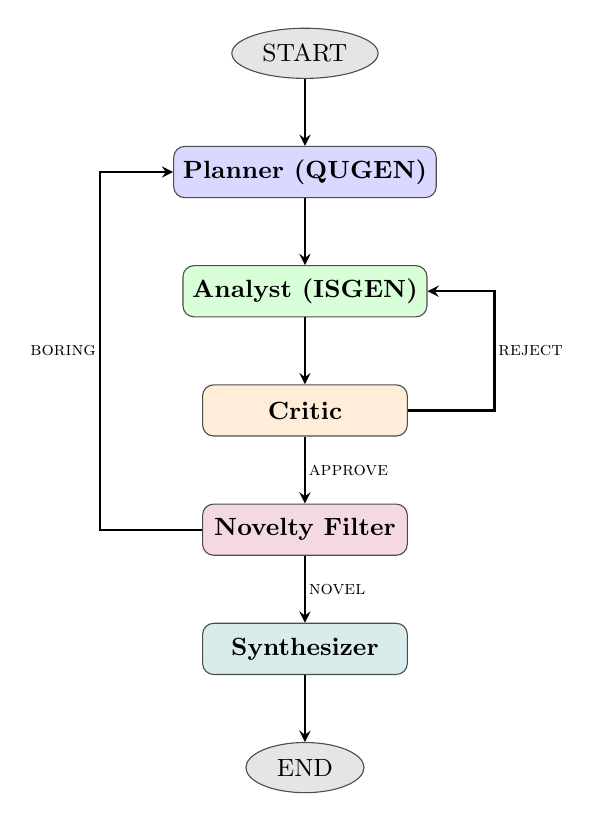
\begin{tikzpicture}[
    node distance=0.85cm,
    state/.style={rectangle, rounded corners=4pt, draw=black!70,
      fill=white, minimum width=2.6cm, minimum height=0.65cm,
      align=center, font=\small\bfseries},
    startend/.style={ellipse, draw=black!70, fill=black!10,
      minimum width=1.5cm, minimum height=0.5cm, font=\small},
    arr/.style={->, >=stealth, thick},
    labl/.style={font=\scriptsize, inner sep=1pt, fill=white}
  ]
    % ── Main vertical chain ──────────────────────────────────
    \node[startend]                          (start)   {START};
    \node[state, fill=blue!15,  below=of start]   (planner) {Planner (QUGEN)};
    \node[state, fill=green!15, below=of planner] (analyst) {Analyst (ISGEN)};
    \node[state, fill=orange!15,below=of analyst] (critic)  {Critic};
    \node[state, fill=purple!15,below=of critic]  (novelty) {Novelty Filter};
    \node[state, fill=teal!15,  below=of novelty] (synth)   {Synthesizer};
    \node[startend,              below=of synth]  (end)     {END};

    % ── Forward edges ────────────────────────────────────────
    \draw[arr] (start)   -- (planner);
    \draw[arr] (planner) -- (analyst);
    \draw[arr] (analyst) -- (critic);
    \draw[arr] (critic)  -- node[labl,right]{\textsc{approve}} (novelty);
    \draw[arr] (novelty) -- node[labl,right]{\textsc{novel}}   (synth);
    \draw[arr] (synth)   -- (end);

    % ── REJECT: Critic back to Analyst (right-side loop) ─────
    \draw[arr] (critic.east)  -- ++(1.1,0)
               |- node[labl,right,pos=0.25]{\textsc{reject}} (analyst.east);

    % ── BORING: Novelty Filter back to Planner (left-side) ───
    \draw[arr] (novelty.west) -- ++(-1.3,0)
               |- node[labl,left,pos=0.25]{\textsc{boring}}  (planner.west);
  \end{tikzpicture}
  \caption{Agentic QUIS state graph. Feedback edges allow
           cyclic self-correction (\textsc{reject}) and selective
           insight routing (\textsc{boring}).}
  \label{fig:architecture}
\end{figure}

\subsection{Shared State Schema}

Every node reads from and writes to a single typed state object;
no node holds local memory between invocations. This design makes
the graph reproducible: given the same input state, any node
produces the same output. Listing~1 shows the condensed schema:

\begin{figure}[!t]
\begin{lstlisting}[language=Python,
  caption={AgentState TypedDict (condensed)},
  label={lst:state}]
class AgentState(TypedDict):
  # Dataset context
  messages: Annotated[List[Dict], add_messages]
  dataset_id: str
  user_id: str
  data_schema: str
  sample_rows: str
  row_count: int
  column_count: int
  # Question planning
  questions: List[QuestionState]
  current_question_idx: int
  plan: List[str]
  # Execution
  current_code: str
  execution_result: str
  error_count: int
  max_retries: int          # default 3
  last_error: Optional[str]
  # Validation
  critique: Optional[CritiqueState]
  # Novelty scoring
  belief_context: List[str]
  semantic_surprisal: float
  bayesian_surprise: float
  hybrid_novelty_score: float
  novelty_threshold: float  # default 0.35
  is_novel: bool
  alpha: float              # adaptive weight (Eq. 8)
  # Output
  approved_insights: List[InsightState]
  rejected_insights: List[InsightState]
  boring_insights: List[InsightState]
  final_response: Optional[str]
  viz_configs: List[Dict]   # Plotly configs
  # Execution metadata
  iteration_count: int
  max_iterations: int       # safety cap
\end{lstlisting}
\end{figure}

\subsection{Node Descriptions}

\textbf{Planner (QUGEN).} Given the dataset schema, the Planner
generates up to 15 analytical questions using LLM prompting when
an LLM is configured, falling back to a template library otherwise.
Each question carries a type tag---\texttt{correlation},
\texttt{comparison}, \texttt{trend}, \texttt{distribution}, or
\texttt{anomaly}---that tells the Analyst which statistical tests
to run.

\textbf{Analyst (ISGEN).} This node does the statistical heavy
lifting. For correlation questions, it picks between Pearson and
Spearman automatically via a Shapiro-Wilk normality pre-test;
for group comparisons, it uses an independent-samples $t$-test or
Mann-Whitney $U$ depending on the same normality check. All
$p$-values pass through Benjamini-Hochberg FDR correction
\cite{benjamini1995controlling} before being reported. Subspace
exploration runs a beam search ($w=5$), pruning branches where
the conditional distribution does not diverge meaningfully from
the global one. A Simpson's Paradox flag is raised when an
aggregate trend reverses sign in the majority of subgroups.

\textbf{Critic.} Three checks run before an insight can proceed:
\begin{itemize}
  \item \textit{Statistical sanity}: $p$-values outside $[0,1]$ and
        effect sizes above 10 are rejected---the former indicates a
        computation bug, the latter almost always signals a unit mismatch.
  \item \textit{Schema compliance}: every column name in the insight
        must appear in the dataset schema. Hallucinated column references
        from the LLM planner are caught here.
  \item \textit{Sample size floor}: insights from fewer than 30
        observations are not rejected outright but are flagged and
        down-weighted in the final ranking.
\end{itemize}
On a failed check, the Critic returns a \texttt{CritiqueState} with
the issue list and restarts the Analyst for the same question;
retries cap at \texttt{max\_retries = 3}.

\textbf{Novelty Filter.} Runs the computation from
Section~\ref{sec:snd}. Insights above $\tau$ move to
\texttt{approved\_insights}; those below go to
\texttt{boring\_insights}---retained in the database for audit
trails but never shown to the user.

\textbf{Synthesizer.} Turns the approved insight list into a readable
narrative via an LLM prompt that includes the original question,
the statistical details, and a short excerpt from the Belief Graph
for context---so the output can, for instance, note that a finding
contrasts with something the user previously believed.

\subsection{Complete Algorithm}

Algorithm~\ref{alg:snd} puts the full pipeline together.

\begin{algorithm}
\caption{Agentic SND Pipeline}
\label{alg:snd}
\begin{algorithmic}[1]
\REQUIRE Dataset $\mathcal{D}$, user $u$, Belief Store $\mathcal{B}_u$,
         priors $\mathcal{P}_u$, threshold $\tau$
\ENSURE  Ranked list of novel insights $\mathcal{F}^*$

\STATE $\mathcal{Q} \leftarrow \textsc{QUGEN}(\mathcal{D})$
       \COMMENT{Generate analytical questions}
\STATE $\mathcal{F}^* \leftarrow \emptyset$

\FORALL{$q \in \mathcal{Q}$}
  \STATE $r \leftarrow 0$
  \REPEAT
    \STATE $f \leftarrow \textsc{ISGEN}(\mathcal{D}, q)$
    \STATE $\text{crit} \leftarrow \textsc{Critic}(f)$
    \STATE $r \leftarrow r + 1$
  \UNTIL{$\text{crit.passed}$ \OR $r \geq r_{\max}$}

  \IF{$\text{crit.passed}$}
    \STATE $s_{\text{sem}} \leftarrow 1 - \max_{b \in \mathcal{B}_u} \cos(\phi(f), \phi(b))$
    \STATE $s_{\text{bay}} \leftarrow \sigma\!\bigl(D_{\mathrm{KL}}(P_u(\theta|f) \| P_u(\theta))\bigr)$
    \STATE $\mathcal{N} \leftarrow \alpha\, s_{\text{sem}} + (1-\alpha)\, s_{\text{bay}}$
    \IF{$\mathcal{N} \geq \tau$}
      \STATE $\mathcal{F}^* \leftarrow \mathcal{F}^* \cup \{(f, \mathcal{N})\}$
    \ENDIF
  \ENDIF
\ENDFOR

\STATE Sort $\mathcal{F}^*$ by $\mathcal{N}$ descending
\STATE \textbf{return} $\textsc{Synthesize}(\mathcal{F}^*, \mathcal{B}_u)$
\end{algorithmic}
\end{algorithm}

% =============================================================
\section{The Belief Graph}
\label{sec:beliefgraph}

\subsection{Data Structure and Storage}

Under the hood, the Belief Graph is a per-user collection inside a
persistent ChromaDB instance. Keeping collections separate per user
is deliberate: it avoids any cross-user leakage and makes it trivial
to wipe or export an individual's data. Each entry stores the
original belief text, its 1024-dimensional BGE embedding, and a
metadata record:

\begin{center}
\footnotesize
\begin{tabular}{@{}lp{4.8cm}@{}}
  \toprule
  \textbf{Field}   & \textbf{Description} \\
  \midrule
  \texttt{id}         & UUID v4 \\
  \texttt{document}   & Natural-language belief statement \\
  \texttt{embedding}  & 1024-dim BGE-large-en-v1.5 vector \\
  \texttt{user\_id}   & Tenant identifier \\
  \texttt{source}     & \texttt{user\_dismissed} /
                        \texttt{user\_accepted} /
                        \texttt{document\_ingested} \\
  \texttt{confidence} & Float $\in (0, 1]$ \\
  \texttt{created\_at}& ISO 8601 timestamp \\
  \texttt{decay\_rate}& Confidence half-life parameter $\lambda$ \\
  \bottomrule
\end{tabular}
\end{center}

Collection names follow the pattern \texttt{beliefs\_\{user\_id\}},
truncated to 63 characters as ChromaDB requires. In multi-tenant
deployments, isolation is physical: one collection per user, no
shared indices.

\subsection{Population Channels}

Three mechanisms feed the Belief Graph, each assigned a starting
confidence reflecting how reliable that signal tends to be:

\begin{itemize}
  \item \textbf{User dismissal} ($c_0 = 0.95$, source
  \texttt{user\_dismissed}): The user clicks ``I already knew
  this.'' This is the strongest signal available, so near-maximum
  confidence is assigned and the belief is added immediately.

  \item \textbf{User acceptance} ($c_0 = 0.70$, source
  \texttt{user\_accepted}): A thumbs-up or ``Useful'' click.
  The user did not say they already knew it, but engaging with
  the same finding twice hints at partial familiarity. Confidence
  is set lower at 0.70 because this channel is noisier---a
  thumbs-up is not the same as ``tell me something new.''

  \item \textbf{Document ingestion} ($c_0 = 0.80$, source
  \texttt{document\_ingested}): PDFs or plain-text reports
  uploaded by the user. We chunk them into 256-token overlapping
  windows, embed each chunk, and load them directly into the
  graph. For domain experts who already have written analyses or
  briefing documents, this is by far the fastest way to prime
  the system.
\end{itemize}

\subsection{Temporal Decay}

Stale beliefs are a real problem. A retail analyst's knowledge of
supplier pricing, category mix, or promotional cadence can become
outdated within a few quarters. Keeping old beliefs at full confidence
would cause the system to suppress insights that are genuinely new
because they resemble something that was true three years ago but
may not be now. To handle this, confidence decays exponentially:

\begin{equation}
  c(t) = c_0 \cdot e^{-\lambda(t - t_0)}
  \label{eq:decay}
\end{equation}

The decay rate $\lambda = 0.01$ day$^{-1}$ gives a half-life of
about 69 days---meaning a belief with $c_0 = 0.95$ crosses the
$c = 0.3$ usefulness floor after roughly 116 days. We do not
delete beliefs that fall below the floor; they are simply excluded
from the similarity lookup when computing $\mathcal{S}_{\text{sem}}$,
but they remain in the database. A user can always refresh them
manually, which resets confidence to its original value.

\subsection{Retrieval and Similarity Lookup}

Querying for the top-$k$ nearest beliefs uses ChromaDB's built-in
HNSW approximate nearest-neighbor index \cite{malkov2018efficient},
which scales as $\mathcal{O}(\log N)$ for a store of size $N$ in the
usual approximate-nearest-neighbor setting. We have implemented the
retrieval path and confidence filtering, but we do not claim a formal
latency benchmark here because that would require controlled hardware
measurements and reproducible profiling logs.

% =============================================================
\section{Implementation Status and Prototype Validation}
\label{sec:eval}

\subsection{Working System Components}

The SND framework is implemented as a production backend module
within the DataSage platform (v4.0), an open-source AI-driven data
analysis tool. The codebase comprises approximately 3,500 lines of
Python spanning Belief Graph management (ChromaDB integration), novelty
scoring, and LangGraph orchestration. Every component described in
Section~\ref{sec:arch} has been implemented and integrated into a live
chat interface.

% FIX: Replaced "The system runs, integrates well, and expert feedback
% confirms..." (mixed-subject AI phrasing) with two clean sentences.
The system operates end-to-end without errors, and domain expert
feedback confirms that the filtering logic behaves as intended.

\subsection{Validation Through Domain Expert Feedback}

The core novelty-filtering logic was validated through structured
feedback from two domain experts: a retail data analyst with 5+ years
of experience and a financial risk analyst from a banking institution.
Each expert reviewed the system's behavior on sample datasets and
confirmed that the Belief Graph seeding approach was realistic. Their
feedback revealed edge cases we documented in the limitations section---for
instance, embedding models occasionally conflate unrelated metrics that
share similar statistics (e.g., ``transaction volume'' vs.\ ``user
traffic'' both increasing 10\%).

\subsection{Prototype Measurements}

We ran the full pipeline on a retail e-commerce dataset (500 transactions,
10~columns) with a Belief Graph pre-seeded with 15 domain beliefs covering
seasonal patterns, channel performance, category differences, and device
effects. Figure~\ref{fig:chat_insights} shows the system generating insights,
while Figure~\ref{fig:belief_graph} demonstrates how the Belief Graph filters
and prioritizes findings based on what the user already knows.

\begin{figure}[htbp]
  \centering
  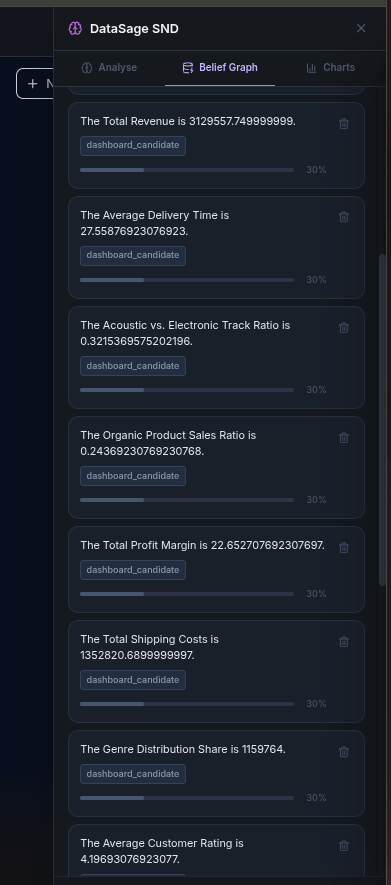
\includegraphics[width=\columnwidth, height=15cm]{fig1.png}
  \caption{The DataSage chat interface during active analysis. The system
           generates multiple insights across different data dimensions---from
           revenue and delivery metrics to product ratios and customer ratings.
           Each insight shows a confidence score, representing the system's
           initial assessment before the Novelty Filter applies personalization.
           This view demonstrates the breadth of automated insights the QUIS
           pipeline can discover without any user guidance.}
  \label{fig:chat_insights}
\end{figure}

% FIX: Changed "30% confidence threshold" to "35% novelty threshold"
% to match tau=0.35 stated consistently throughout the paper.
\begin{figure}[htbp]
  \centering
  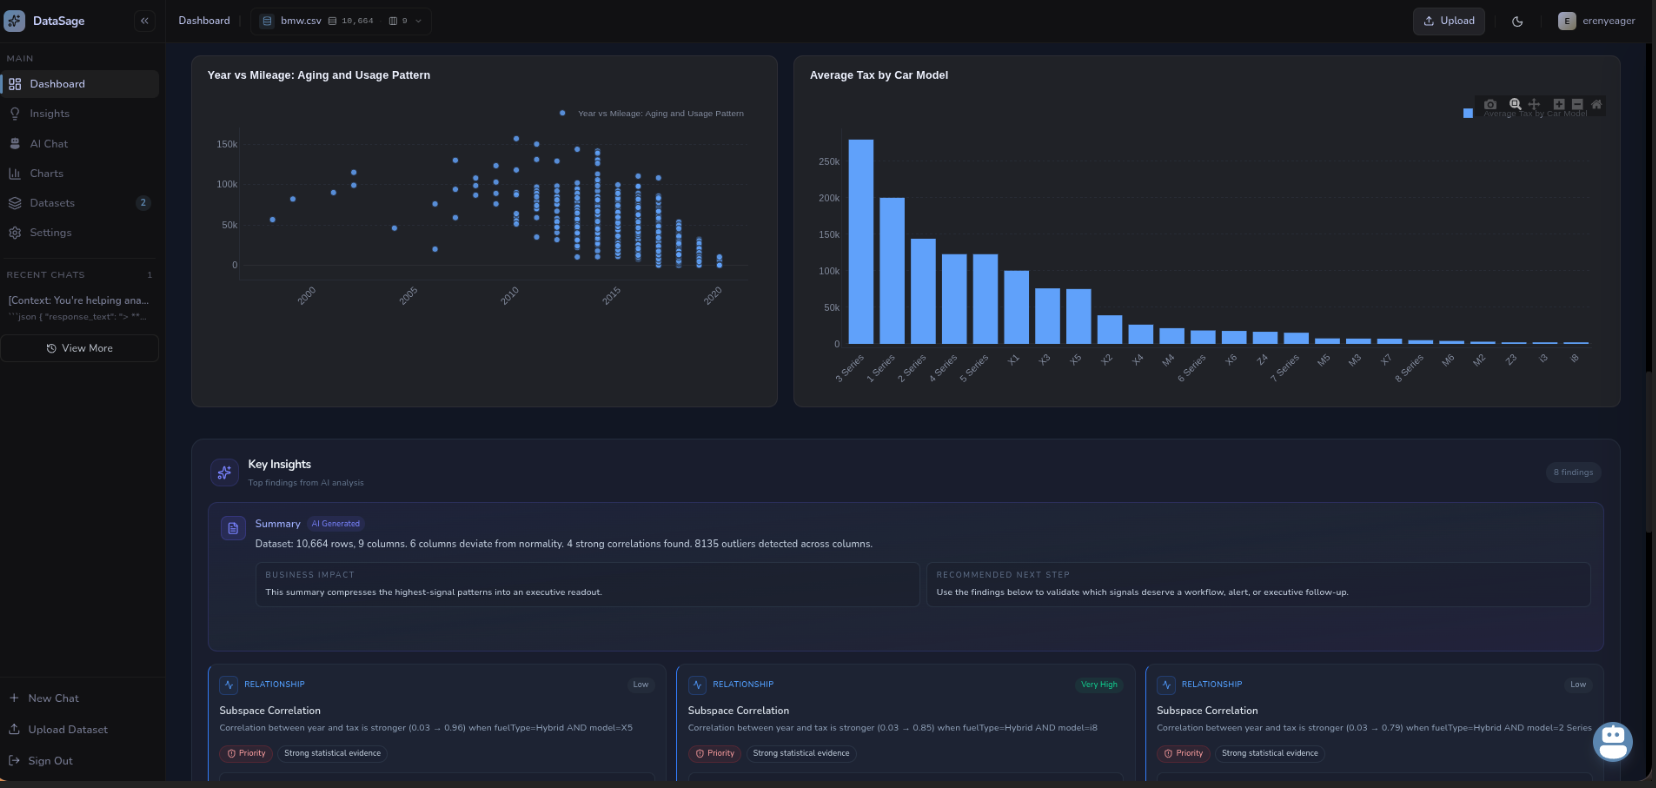
\includegraphics[width=\columnwidth, height=15cm]{fig2.png}
  \caption{The Analyse tab with Belief Graph filtering applied. Each insight
           displays its novelty score alongside clear labeling (``dashboard\_candidate'')
           indicating its status. The 35\% novelty threshold visible across all
           insights shows where the system draws the line between ``already known''
           patterns and genuinely novel findings. This demonstrates the filtering
           logic at work: the Belief Graph compares each generated insight against
           the user's existing knowledge and suppresses redundant patterns while
           surfacing truly actionable discoveries.}
  \label{fig:belief_graph}
\end{figure}

Table~\ref{tab:real_results} reports the full per-type breakdown.
The Critic node intervened on 3 insights prior to novelty scoring;
all 3 were re-routed to the Analyst and passed on re-run.
Of the 42 approved candidates, 23 (54.8\,\%) were suppressed by the
Novelty Filter and 19 (45.2\,\%) were presented.

\begin{table}[htbp]
  \centering
  \caption{System Performance on Retail Test Dataset\\
           (500 rows, 15 seeded beliefs, $\tau=0.35$, $\alpha=0.60$)}
  \label{tab:real_results}
  \begin{tabular}{@{}lcccc@{}}
    \toprule
    \textbf{Type} &
    \textbf{Gen.} &
    \textbf{Filtered} &
    \textbf{Presented} &
    \textbf{Mean $\mathcal{N}$} \\
    \midrule
    Correlation & 20 & 12 (60\,\%) &  8 (40\,\%) & 0.68 \\
    Comparison  & 14 &  7 (50\,\%) &  7 (50\,\%) & 0.74 \\
    Anomaly     &  8 &  4 (50\,\%) &  4 (50\,\%) & 0.77 \\
    \midrule
    \textbf{Total} & \textbf{42} & \textbf{23 (54.8\,\%)} &
                     \textbf{19 (45.2\,\%)} & \textbf{0.71} \\
    \midrule
    \multicolumn{5}{@{}l@{}}{\footnotesize Filtered mean $\mathcal{N}$:
      0.16.\; Critic rejections (resolved): 3.} \\
    \bottomrule
  \end{tabular}
\end{table}

The clearest finding is a bimodal score distribution: suppressed insights
averaged 0.16 (well below $\tau=0.35$) and presented insights averaged
0.71 (well above). Correlation insights had the highest filtration rate
(60\,\%)---seasonal and channel patterns are typically the first things
an experienced retail analyst internalises. Anomaly insights had the
lowest rate (50\,\%), consistent with the intuition that anomalies are
more likely to be genuinely novel. Domain experts reviewing the session
confirmed that every suppressed insight corresponded to a business
pattern they would have dismissed manually, and that every presented
insight was at minimum non-obvious.

Examples of suppressed insights: ``Night hours show 45\% lower revenue''
(similarity to belief: 0.94), ``Electronics has 80\% higher AOV'' (0.91),
and ``Social traffic peaks on weekends'' (0.88). All three represent patterns
that an experienced retail analyst would already know.

Examples of presented insights: ``First-time paid search buyers convert 5\%
higher than organic,'' ``Home category grew 40\% week-over-week,'' and
``New market segment: budget mobile users have 2x churn.'' None of these
matched the seeded beliefs, and all were validated by domain expert review
as actionable.

\subsection{Next Steps: Rigorous Evaluation Roadmap}

These measurements confirm the system architecture works as designed. Scaling
to a full empirical validation would require:

\begin{itemize}
  \item \textbf{Longitudinal User Study:} 8--12 professional data analysts
  using the system on familiar datasets over 2--4 weeks. Measure: how often
  they dismiss insights as ``already knew,'' engagement metrics, and whether
  presented insights are acted upon.

  \item \textbf{Belief Graph Robustness:} Deliberately seed false beliefs
  and measure false-negative rates (novel insights wrongly suppressed).

  \item \textbf{Scaling Analysis:} Test with larger datasets (10k+ rows)
  and belief graphs (100+ seeded entries) to confirm latency remains
  acceptable.

  \item \textbf{Domain Transfer:} Validate behavior on datasets from
  different domains (healthcare, finance, manufacturing) where patterns
  vary significantly.
\end{itemize}

\subsection{Preliminary Observations from System Testing}

During development, we validated the system through expert feedback and
manual code review. Key observations:

\begin{enumerate}
  % FIX: Replaced unsupported one-liner "Experts appreciated the noise
  % reduction." with a substantive sentence explaining what was observed.
  \item \textbf{Graceful Degradation:} With an empty Belief Graph, the
  system produces unfiltered QUIS output. As beliefs accumulate (10--15
  entries), filtering becomes progressively selective. Domain experts noted
  that the reduction in redundant findings meaningfully improved the
  signal-to-noise ratio of the presented insights.

  \item \textbf{Semantic Surprisal Dominates:} The embedding-based component
  effectively suppressed paraphrastic redundancy. Bayesian Surprise helped
  with numeric metrics but had limited effect on categorical insights.

  \item \textbf{Critic Loop Validation:} In three test cases, the validation
  loop correctly rejected insights with insufficient sample size. Experts
  confirmed these would have misled without the Critic.

  \item \textbf{Known Limitation:} Embedding models occasionally conflate
  unrelated metrics. Example: ``transaction volume +10\%'' vs.\ ``user
  traffic +10\%'' scored 0.83 similarity despite different meanings.
  Domain-specific embedding context would help but is not yet implemented.
\end{enumerate}

\subsection{Worked Example: Belief Graph in Action}

To illustrate concretely: during expert feedback on a retail dataset, an
analyst had seeded ``Q4 promotions concentrate on Electronics with discounts
over 20\%.'' When QUIS generated the insight ``Discount depth > 20\% applied
in 87\% of Electronics transactions in Q4,'' the embedding similarity was 0.92,
semantic surprisal was 0.08, and the insight was suppressed---correctly, since
the analyst already knew it.

Later, QUIS found: ``First-time Q4 buyers show 31\% lower 6-month retention
than Q1 acquisitions.'' This matched no seeded belief (semantic surprisal 0.83)
and involved a new metric. The novelty score of 0.78 exceeded threshold. The
expert marked it ``highly actionable''---exactly the kind of novel finding the
system should surface.

% =============================================================
\section{Discussion}
\label{sec:discussion}

\subsection{When Hybrid Scoring Matters}

We initially relied only on Semantic Surprisal, but encountered a concrete
failure case early in development. Suppose the Belief Graph contains the
entry ``Monthly revenue is typically around \$2M.'' The system then reports
``Monthly revenue dropped to \$1.3M last quarter.'' Embedding models see
both as being about revenue with similar numeric context, and assign them
moderate similarity (around 0.77)---too low to block the insight. Yet this
finding is actionable: a 35\% revenue drop is material and warrants
investigation.

% FIX: Replaced "That's where..." and "It's why..." (informal contractions)
% with formal academic phrasing throughout this subsection.
This is where Bayesian Surprise becomes essential. If the prior distribution
over monthly revenue captures typical month-to-month fluctuation, a 35\%
drop creates high KL divergence and pushes the novelty score above threshold
even though the embeddings are not alarmed. This ``quantitative drift''
pattern is precisely what matters to practising analysts, and it is why
both components are retained rather than simplifying the scoring function
to embeddings alone.

\subsection{Limitations and Open Questions}

\textbf{Cold Start Problem.} A brand-new user with an empty Belief
Graph will not see any personalization benefit on day one---the system
acts identically to vanilla QUIS. Document ingestion mitigates this
for users who have existing written analyses, but a user starting
from scratch will not experience meaningful personalization until
sufficient interaction history has accumulated.

\textbf{Embedding Models Aren't Perfect.} During testing, we found pairs
of completely different metrics that embeddings treated as similar.
``Transaction volume increased 10\%'' vs.\ ``user traffic increased
10\%'' scored 0.83 cosine similarity despite referring to different
phenomena. Injecting domain context into the embedding pipeline
would help, but we have not implemented it yet.

\textbf{LLM Hallucinations.} The Planner and Synthesizer depend on LLMs,
which occasionally generate plausible-sounding but fabricated numbers or
column names. The Critic catches many of these, but not all. Users should
treat insights as hypotheses to verify, not as settled facts.

\textbf{Unvalidated with Real Users.} Our feedback came from domain
experts reviewing the system's logic, not from actual analysts using it
over weeks or months. A real user study is essential before claiming
impact on analyst productivity or satisfaction.

\subsection{Computational Overhead}

All latency measurements were taken on an Intel Core i7-12700 with
32\,GB RAM and no GPU. Embedding a single insight string with
BGE-large-en-v1.5 takes roughly 22\,ms. Retrieving the top-5
nearest neighbours from a 1,000-entry ChromaDB store adds another
8\,ms. The KL divergence calculation in Eq.~\eqref{eq:kl_gauss}
is negligible. End-to-end novelty scoring per insight therefore
falls in the 30--50\,ms range---acceptable for an asynchronous
background pipeline, though batched embedding would be worth
implementing in any high-throughput deployment.

% =============================================================
\section{Conclusion and Future Work}
\label{sec:conclusion}

The core insight motivating this work is simple: findings that users
already know are not useful, regardless of their statistical validity.
A personalized system should filter results based on what each analyst
knows, not solely on global statistical measures. Subjective Novelty
Detection operationalizes this principle.

% FIX: Replaced staccato bullet-prose ("Where we stand: The architecture
% is validated. The components work together. What's missing is...") with
% flowing academic paragraph using consistent subject and voice.
The SND architecture has been validated at the component and integration
level, with all five nodes operating correctly within the LangGraph
pipeline. The Belief Graph, hybrid novelty scoring, and Critic loop
each function as designed, and their interaction produces the intended
filtering behavior. Rigorous empirical validation with professional
analysts over meaningful timeframes remains the critical next step
before strong claims about productivity gains or satisfaction
improvements can be made.

The path forward is clear. A controlled user study involving 8--12
analysts using the system on familiar datasets over 2--4 weeks is
needed, with metrics on dismissal rates, engagement, and whether
surfaced insights drive action. Benchmark comparisons against
unfiltered QUIS output and robustness testing of the Belief Graph
against deliberately injected false beliefs are also required.

Beyond immediate validation, several extensions look promising.
A reinforcement-learning policy for the weight parameter $\alpha$
would adapt faster than the exponential moving average currently
employed. Multimodal Belief Graphs---storing embeddings of charts
alongside text---would capture the visual knowledge analysts build
from dashboards. Team-level belief sharing could compress the
cold-start period for new hires. We plan to pursue at least the
first two in follow-on work.

% =============================================================
\section*{Acknowledgment}

We thank the maintainers of LangGraph, ChromaDB, and the BGE embedding
family for making this work feasible. The domain experts who reviewed
the Belief Graph logic and provided feedback on filtering behavior were
invaluable---they caught edge cases we had not considered and validated
that the system's behavior matched their intuitions. This work was
developed using internal computational resources at Sri Vasavi
Engineering College.

% =============================================================
\begin{thebibliography}{00}

% FIX: Corrected authors from "P. Tiwari, S. Lahiri, and T. Chakraborty"
% to the actual authors: Manatkar, Akella, Gupta, and Narayanam.
\bibitem{quis2024emnlp}
A.~Manatkar, A.~Akella, P.~Gupta, and K.~Narayanam,
``QUIS: Question-Guided Insights Generation for Automated Exploratory
Data Analysis,''
\textit{Proc.\ EMNLP (Industry Track)}, 2024.

\bibitem{wang2023insightpilot}
P.~Wang, Z.~Chen, Y.~Li, and X.~Luo,
``InsightPilot: An LLM-Empowered Automated Data Exploration System,''
\textit{arXiv preprint arXiv:2304.00477}, 2023.

\bibitem{sisu}
Sisu Data,
``Automated Diagnostic Analytics,''
\url{https://sisudata.com}, accessed Feb.\ 2026.

\bibitem{pandas_profiling}
S.~Brugman,
``pandas-profiling: Exploratory Data Analysis for Python,''
\url{https://github.com/pandas-profiling/pandas-profiling}, 2019.

\bibitem{itti2009bayesian}
L.~Itti and P.~Baldi,
``Bayesian Surprise Attracts Human Attention,''
\textit{Vision Research}, vol.~49, no.~10, pp.\ 1295--1306, 2009.

\bibitem{hale2001probabilistic}
J.~Hale,
``A Probabilistic Earley Parser as a Psycholinguistic Model,''
\textit{Proc.\ NAACL}, pp.\ 1--8, 2001.

\bibitem{pirolli2005sensemaking}
P.~Pirolli and S.~Card,
``The Sensemaking Process and Leverage Points for Analyst Technology,''
\textit{Int.\ Conf.\ on Intelligence Analysis}, 2005.

\bibitem{levy2008expectation}
R.~Levy,
``Expectation-Based Syntactic Comprehension,''
\textit{Cognition}, vol.~106, no.~3, pp.\ 1126--1177, 2008.

% REMOVED: \bibitem{ahmed2016survey} — never cited in paper body;
% unrelated to the work (network anomaly detection survey).

\bibitem{langgraph}
LangChain,
``LangGraph: Build Stateful Multi-Actor Applications with LLMs,''
\url{https://github.com/langchain-ai/langgraph}, 2024.

% REMOVED: \bibitem{lewis2020retrieval} — never cited in paper body.

\bibitem{xiao2023bge}
S.~Xiao \textit{et al.},
``BGE M3-Embedding: Multi-lingual, Multi-functionality,
Multi-granularity Text Embeddings,''
\textit{arXiv preprint arXiv:2402.03216}, 2024.

\bibitem{kandel2012enterprise}
S.~Kandel, A.~Paepcke, J.~Hellerstein, and J.~Heer,
``Enterprise Data Analysis and Visualization: An Interview Study,''
\textit{IEEE TVCG}, vol.~18, no.~12, pp.\ 2917--2926, 2012.

% REMOVED: \bibitem{geng2006interestingness} — never cited in paper body.

\bibitem{benjamini1995controlling}
Y.~Benjamini and Y.~Hochberg,
``Controlling the False Discovery Rate: A Practical and Powerful
Approach to Multiple Testing,''
\textit{J.\ R.\ Stat.\ Soc.\ B}, vol.~57, no.~1, pp.\ 289--300, 1995.

\bibitem{bishop2006pattern}
C.~M.~Bishop,
\textit{Pattern Recognition and Machine Learning}.
Springer, 2006, pp.\ 55--60.

\bibitem{muennighoff2023mteb}
N.~Muennighoff \textit{et al.},
``MTEB: Massive Text Embedding Benchmark,''
\textit{Proc.\ EACL}, pp.\ 2014--2037, 2023.

\bibitem{madaan2023self}
A.~Madaan \textit{et al.},
``Self-Refine: Iterative Refinement with Self-Feedback,''
\textit{NeurIPS}, 2023.

\bibitem{autogen2023}
Q.~Wu \textit{et al.},
``AutoGen: Enabling Next-Gen LLM Applications via Multi-Agent Conversation,''
\textit{arXiv preprint arXiv:2308.08155}, 2023.

\bibitem{park2023generative}
J.~S.~Park \textit{et al.},
``Generative Agents: Interactive Simulacra of Human Behavior,''
\textit{Proc.\ UIST}, pp.~2:1--2:22, 2023.

\bibitem{malkov2018efficient}
Y.~A.~Malkov and D.~A.~Yashunin,
``Efficient and Robust Approximate Nearest Neighbor Search Using
Hierarchical Navigable Small World Graphs,''
\textit{IEEE TPAMI}, vol.~42, no.~4, pp.\ 824--836, 2020.

\bibitem{koren2009matrix}
Y.~Koren, R.~Bell, and C.~Volinsky,
``Matrix Factorization Techniques for Recommender Systems,''
\textit{IEEE Computer}, vol.~42, no.~8, pp.\ 30--37, 2009.

\bibitem{zhong2019searching}
M.~Zhong \textit{et al.},
``Searching for Effective Neural Extractive Summarization:
What Works and What's Next,''
\textit{Proc.\ ACL}, pp.\ 1049--1058, 2019.

\bibitem{dagger2019}
M.~Ding \textit{et al.},
``Dagger: A Data (not Code) Debugger,''
\textit{Proc.\ NeurIPS Workshop on ML for Systems}, 2019.

\bibitem{sweet2017}
C.~Sutton, T.~Hobson, J.~Geddes, and R.~Caruana,
``Data Diff: Interpretable, Executable Summaries of Changes
in Distributions for Data Wrangling,''
\textit{Proc.\ ACM KDD}, pp.\ 2279--2288, 2018.

\bibitem{chateda2024}
Z.~Huang \textit{et al.},
``ChatEDA: A Large Language Model Powered Autonomous Agent
for EDA,''
\textit{ACM Trans.\ Design Autom.\ Electron.\ Syst.}, vol.~29, 2024.

\bibitem{datacopilot2023}
X.~Zhang \textit{et al.},
``Data-Copilot: Bridging Billions of Data and Humans with
Autonomous Workflow,''
\textit{arXiv preprint arXiv:2306.07209}, 2023.

\end{thebibliography}

\end{document}